\subsection{Polynomial functions from x-intercepts and graphs}
\begin{definition}[Zero Product Property]
  If the product two numbers or expressions is \textit{zero}, then at least \textit{one} those factors must be \textit{zero}.
\end{definition}

\begin{definition}[Polynomial functions from x-intercepts and graphs]
  Making a polynomial function from x intercepts of a function or graphs of a function.
\end{definition}

\begin{example}[Polynomial functions from x-intercepts]
  \hfill
  \begin{enumerate}
  \item Suppose $x$-intercept $-3, 4, 1, + 0$ \\
    $x = -3 \quad x = 4 \quad x = 1 \quad x = 0$ \\
    $x + 3 = 0 \quad x + -4 = 0 \quad x - 1 = 0 \quad x = 0$ \\
    $x(x + 3)(x - 4)(x - 1) = 0$ \\
    $f(x) = ax(x + 3)(x - 4)(x - 1)$ \\
    \textbf{Note: }Zeros here is the $x$-intercepts.
  \item Zeros: $-1, 0, 4, -9$. Degree $4$ polynomial. \\
    $x = -1 \quad x = 0 \quad x = 4 \quad x = -9$ \\
    $x + 1 = 0 \quad x = 0 \quad x - 4 = 0 \quad x + 9 = 0$ \\
    $x(x + 1)(x - 4)(x + 9) = 0$ \\
    $f(x) = ax(x + 1)(x - 4)(x + 9)$
  \item Zeros: $1 \text{ mult } 1, \, 2 \text{ mult } 2$. Degree 3 polynomial.
    $x = 1 \quad x = 2$ \\
    $x - 1 = 0 \quad x - 2 = 0$ \\
    $(x - 1)(x - 2)^2 = 0$ \\
    $f(x) = a(x - 1)(x - 2)^2$
  \item Zeros: $-1 \text{ mult } 2, \, 5 \text{ mult } 1, \, 0 \text{ mult } 3, \, \frac{1}{2} \text{ mult } 3$. Degree 9 polynomial. \\
    $x = -2 \quad x = 5 \quad x = 0 \quad x = \frac{1}{2}$ \\
    $x + 2 = 0  \quad x - 5 = 0 \quad x = 0 \quad x - \frac{1}{2} = 0$ \\
    $x^3(x + 2)^2(x - 5)(x - \frac{1}{2})^3 = 0$ \\
    $f(x) = ax^3(x + 2)^2(x - 5)(x - \frac{1}{2})^3$ 
  \end{enumerate}
\end{example}

\textbf{Note: }The degree is always at least one more than the turning point.

\begin{example}[Polynomial functions from graphs]
  \hfill
  \begin{enumerate}
  \item \hfill
    \begin{center}
      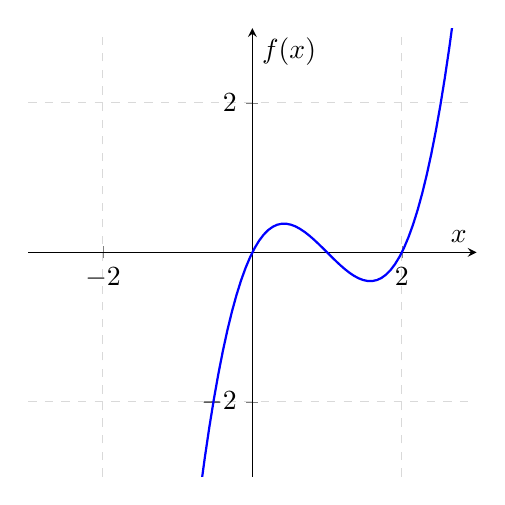
\begin{tikzpicture}
        \begin{axis}[
	    axis lines = center,
	    xlabel = $x$,
	    ylabel = $f(x)$,
	    xmin = -3, xmax = 3,
	    ymin = -3, ymax = 3,
            restrict y to domain = -20:10,
	    grid = major,
	    grid style = {dashed, gray!30},
	    axis equal image
	  ]
	  \addplot [domain=-3:3, samples=100, thick, blue] {x*(x-1)*(x-2)};
        \end{axis}
      \end{tikzpicture}
    \end{center}
    $x = 0 \quad x = 1 \quad x = 2$ \\
    $x = 0 \quad x - 1 = 0 \quad x - 2 = 0$ \\
    $x(x - 1)(x - 2) = 0 $ \\
    $f(x) = ax(x - 1)(x - 2)$
  \item \hfill
    \begin{center}
      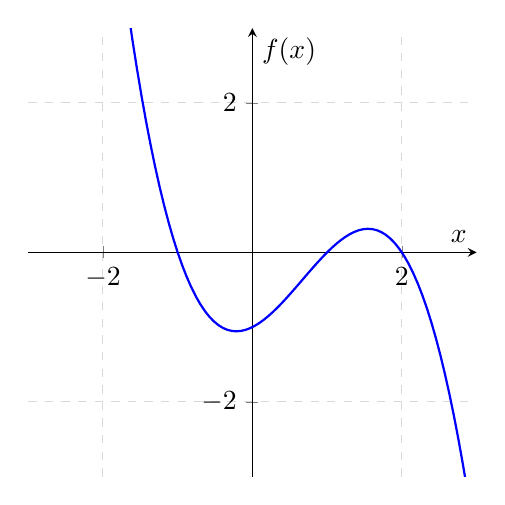
\begin{tikzpicture}
        \begin{axis}[
	    axis lines = center,
	    xlabel = $x$,
	    ylabel = $f(x)$,
	    xmin = -3, xmax = 3,
	    ymin = -3, ymax = 3,
            restrict y to domain = -20:10,
	    grid = major,
	    grid style = {dashed, gray!30},
	    axis equal image
	  ]
	  \addplot [domain=-3:3, samples=100, thick, blue] {-0.5*(x+1)*(x-1)*(x-2)};
        \end{axis}
      \end{tikzpicture}
    \end{center}
    $(0, -1)$ \\
    $x = - 1 \quad x = 1 \quad x = 2$ \\
    $x + 1 = 0 \quad x - 1 = 0 \quad x - 2 = 0$ \\
    $f(x) = a(x + 1)(x - 1)(x - 2)$ \\
    $-1 = a(0 + 1)(0 - 1)(0 - 2)$ \\
    $-1 = a(1)(-1)(-2)$ \\
    $-1 = 2a$ \\
    $-\frac{1}{2} = a$ \\
    $f(x) = -\frac{1}{2}(x + 1)(x - 1)(x - 2)$
  \item \hfill
    \begin{center}
      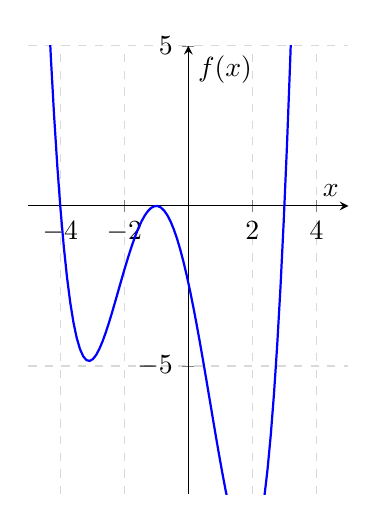
\begin{tikzpicture}
        \begin{axis}[
	    axis lines = center,
	    xlabel = $x$,
	    ylabel = $f(x)$,
	    xmin = -5, xmax = 5,
	    ymin = -9, ymax = 5,
            restrict y to domain = -20:10,
	    grid = major,
	    grid style = {dashed, gray!30},
	    axis equal image
	  ]
	  \addplot [domain=-5:5, samples=100, thick, blue] {0.2*(x+4)*(x + 1)^2*(x - 3)};
        \end{axis}
      \end{tikzpicture}
    \end{center}
    $(1, -8)$ \\
    $x = -4 \quad x - 1 \quad x = 3$ \\
    $x + 4 = 0 \quad x + 1 = 0 \quad x - 3 = 0$ \\
    $(x + 4)(x + 1)^2(x - 3) = 0$ \\
    $f(x) = a(x + 4)(x + 1)^2(x - 3)$ \\
    $-8 = a(1 + 4)(1 + 1)^2(1 - 3)$ \\
    $-8 = a(5)(2)^2(-2)$ \\
    $-8 = a \cdot 5 \cdot 4 \cdot (-2)$ \\
    $-8 = 40a$ \\
    $\frac{1}{5} = a$ \\
    $f(x) = \frac{1}{5}(x + 4)(x + 1)^2(x - 3)$
  \end{enumerate}
\end{example}
